\documentclass[10pt,a4paper]{article}
\usepackage[utf8]{inputenc}
\usepackage{amsmath}
\usepackage{amsfonts}
\usepackage{amssymb}
\usepackage{graphicx}
\usepackage{subfigure}
\usepackage{amsmath}
\usepackage{mathrsfs}
\DeclareRobustCommand{\orderof}{\ensuremath{\mathcal{O}}}
\bibliographystyle{prsty}
\usepackage[top=1in, bottom=1in, left=1in, right=1in]{geometry}
\begin{document}
\section{Introduction}
\textbf{lat} file generates the lattice structure of a given systems. A lattice is constructed by three parameters: 1). lattice constant 2). primitive lattice vectors 3). sublattice vectors. Any lattice site is specified by four index $[n_{1},n_{2},n_{3},s]$ which follows the rules: $\textbf{r}_{s}^{n_{1},n_{2},n_{3}}=n_{1}\textbf{a}_{1}+n_{2}\textbf{a}_{2}+n_{3}\textbf{a}_{3}+\textbf{d}_{s}$, where $[n_{1},n_{2},n_{3}]$ are integers which specifies the unitcell and $d_{s}$ specifies the sublattice vectors. If there are $N$ sublattices in a unitcell, then $s$ ranges from 1 to $N$. In this task, users have to input all necessary parameters and PiLab will search for the nearest neighbor sites of a sublattice in the $[n_{1}=0,n_{2}=0,n_{3}=0]$ unitcell up to $n$-th order.

\section{Dictionary}

\subsection{Input}
\textit{\textbf{lat.Const}} This parameter sets the lattice constant of the system. The values of lat.Primitive and lat.Sublattice will automatically multiply this parameter during the calculation. \\ \\
\textit{\textbf{lat.Primitive}} This parameter sets the primitive lattice vectors. This parameter multiply lat.Const defines the $[\textbf{a}_{1},\textbf{a}_{2},\textbf{a}_{3}]$ vectors. Each lattice vector is represented by a row vector $x,y,z$ and different vectors are separated by a semicolon ";" as shown in Fig.1. If the system is two or one dimension, each row vector can be given by two or one dimension only. For example, the primitive lattice vector of a 2D graphene can be: $[-3/2,sqrt(3)/2;3/2,sqrt(3)/2]$ ("sqrt" is the keyword of square root in Scilab). For 1D dimer chain, it can be $[1]$ \\ \\
\textit{\textbf{lat.Sublatt}} This parameter sets the sublattice vectors. This parameter multiply lat.Const defines the $\textbf{d}_{s}$ vectors. Also, different vectors are separated by semicolons ";". \\ \\
\textit{\textbf{lat.Order}} This parameter sets the order of neareat neighbor. For example, lat.Order=[2] means PiLab will search first and second order of nearest neighbor sites of each sublattice located in the $[n_{1}=0,n_{2}=0,n_{3}=0]$ unitcell. 

\subsection{Output}
\textit{\textbf{lat.recip\_vec}} This variable gives you the reciprocal lattice vectors, $\textbf{b}_{1}=2\pi \frac{\textbf{a}_{2}\times \textbf{a}_{3}}{\textbf{a}_{1} \cdot (\textbf{a}_{2}\times \textbf{a}_{3})}$, $\textbf{b}_{2}=2\pi \frac{\textbf{a}_{3}\times \textbf{a}_{1}}{\textbf{a}_{2} \cdot (\textbf{a}_{3}\times \textbf{a}_{1})}$, $\textbf{b}_{3}=2\pi \frac{\textbf{a}_{1}\times \textbf{a}_{2}}{\textbf{a}_{3} \cdot (\textbf{a}_{1}\times \textbf{a}_{2})}$. In Fig.3, PiLab gives you a 3x3 matrix. Each row vectors corresponds to a reciprocal lattice vector. \\ \\
\textit{\textbf{lat.surr\_site(n)}} This variable gives you the surrounding neighbor sites of the n-th sublattice. For example, lat.surr\_site(1) gives you the surrounding neighbor sites of sublattice 1 defined by the first row vector in lat.Sublatt. There are nine values of each row vector whose meaning is [order, distance, sublattice index, $n_{1}$, $n_{2}$, $n_{3}$, x, y, z].  The sublattice itself will always listed in the first row, so the order is always 0 and distance is always 0 too. Therefore, in Fig.1, the third row vector of lat.surr\_site(1) means there is a first order neighbor site around sublattice 1. The distance between them is 0.5 and this neighbor site belongs to sublattice 2. It is located in the [$n_{1}=-1$, $n_{2}=0$, $n_{3}=-1$] unitcell and its coordinate is [0,-0.5,0]. One should check this variable carefully to make sure the lattice structure is generated correctly. If not, you might pick wrong primitive lattice vectors or sublattice vectors.

\begin{figure}[tbp]
\centering
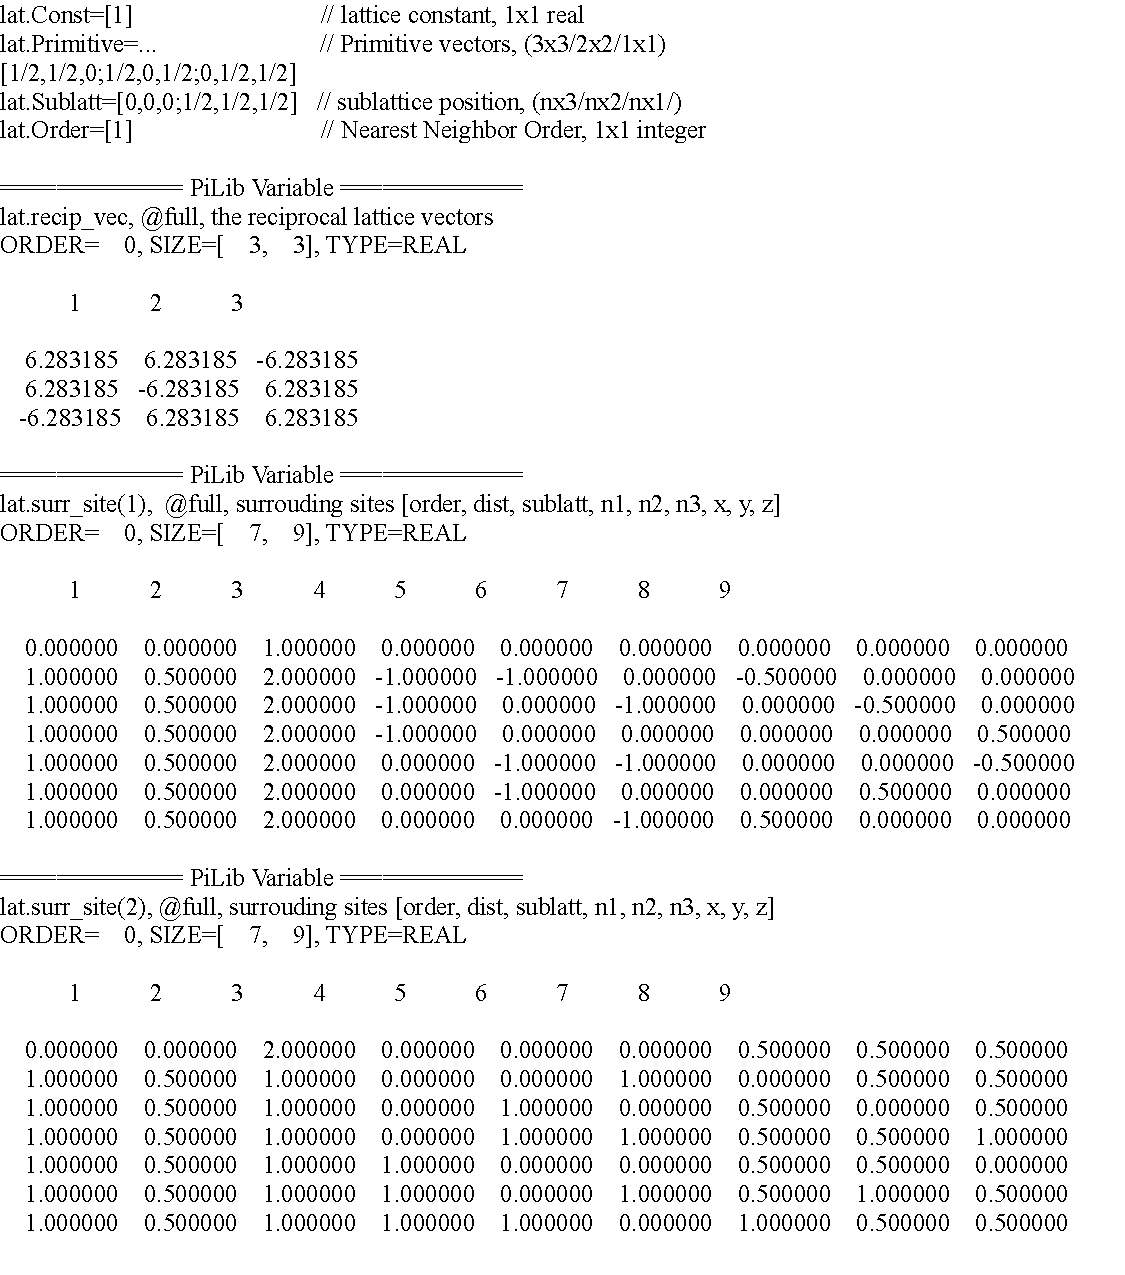
\includegraphics[width=1.0\columnwidth]{NiO_lat.pdf}
\caption{NiO\_lat.plb}
\end{figure}


\end{document}